\documentclass[11pt,a4paper]{article}
\usepackage[hyperref]{emnlp2018}
\usepackage{times}
\usepackage{latexsym}
\usepackage{amsmath}
\usepackage{amsthm}
\usepackage{framed}
\usepackage{caption}
\usepackage{subcaption}
\usepackage{graphicx}
\usepackage{xcolor,colortbl}
\usepackage{algorithm2e}
\usepackage{url}
 \usepackage{multirow}
\usepackage{tikz}
\usetikzlibrary{calc, positioning, arrows, automata,fit,shapes.geometric,backgrounds,shapes.misc}
\usepackage{tikz-dependency}
\usepackage{pgfplots}
\pgfplotsset{compat=1.12}
\newcommand\BibTeX{B{\sc ib}\TeX}
%\def\aclpaperid{254} %  Enter the acl Paper ID here
\aclfinalcopy

%\title{Informative Linguistic Features as Saviors for Coreference Generalization}
\title{Using Linguistic Features to Improve Generalization \\in Neural Coreference Resolvers}

\date{}

\begin{document}
\maketitle

\appendix
\section{Supplemental Material}
\label{sec:supplemental}

\subsection{Running Example for FP-Tree Construction}
Assume $D$ contains the following three samples:
\begin{itemize}
 \item [] $X_1$=\{ana-type=NAM, ant-type=NAM, head-match=F\}, $C(X_1)=0$
 \item[]  $X_2$=\{ana-type=NAM, ant-type=NAM, head-match=T\}, $C(X_2)=1$
 \item[]  $X_3$=\{ana-type=NAM, ant-type=NOM, head-match=F\}, $C(X_3)=0$
 %\item[]  $X_4$=\{ana-type=nominal, ana-number=singular, ante-type=nominal, ante-number=singular}\}, $C(X_4)=1$
\end{itemize}
Based on these three samples
\begin{itemize}
\item $A$=\{ana-type=NAM, ant-type=NAM, head-match=F, head-match=T, ant-type=NOM\},
\item $support(a_i,0)_{a_i \in A}$= \{2,1,2,0,1\}, e.g.\ ``ana-type=NAM'' appeared two times in non-coreferring ($C(X_i)=0$) samples,
\item and $support(a_i,1)_{a_i \in A}$=\{1,1,0,1,0\}.
\end{itemize}
If we sort $A$ based on $a_i$'s frequencies, i.e. $support(a_i,0)+support(a_i,1)$, the ordering of $A$'s items will remain the same.

Now, we need to go through the samples again to build the tree.
The FP-Tree construction steps after adding each of the above samples is demonstrated in Figure~\ref{fp-tree_example}.
ana-type=NAM, ant-type=NAM, head-match=F, head-match=T, and ant-type=NOM are abbreviated as
ana=NAM, ant=NAM, head=F, head=T, and ant=NOM, respectively in Figures~\ref{fp-tree_example} and ~\ref{final-fp-tree_example}.
%
\begin{figure*}[!htb]
\minipage{0.28\textwidth}
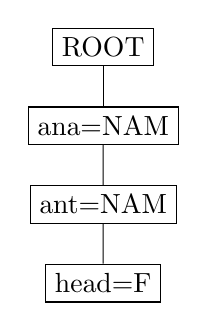
\begin{tikzpicture}
\node [rectangle,draw]{ROOT} [level distance=10mm,sibling distance=30mm]
child { node [rectangle,draw]{ana=NAM} [level distance=10mm ,sibling distance=15mm]
child {node [rectangle,draw] {ant=NAM}
child {node [rectangle,draw] {head=F}
}}};
\end{tikzpicture}
\endminipage\hfill
\minipage{0.28\textwidth}
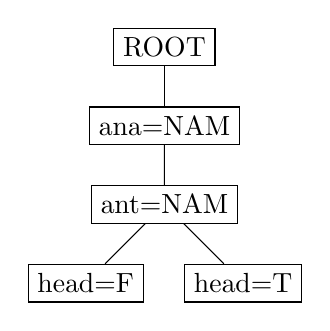
\begin{tikzpicture}
\node [rectangle,draw]{ROOT} [level distance=10mm,sibling distance=30mm]
child { node [rectangle,draw]{ana=NAM} [level distance=10mm ,sibling distance=20mm]
child {node [rectangle,draw] {ant=NAM}
child {node [rectangle,draw] {head=F}}
child {node [rectangle,draw] {head=T}}
}};
\end{tikzpicture}
\endminipage\hfill
\minipage{0.37\textwidth}%
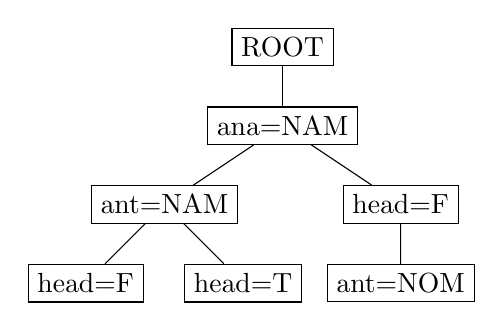
\begin{tikzpicture}
\node [rectangle,draw]{ROOT} [level distance=10mm,sibling distance=25mm]
child { node [rectangle,draw]{ana=NAM} [level distance=10mm ,sibling distance=30mm]
child {node [rectangle,draw] {ant=NAM}  [level distance=10mm ,sibling distance=20mm]
child {node [rectangle,draw] {head=F}}
child {node [rectangle,draw] {head=T}}
}
child {node [rectangle,draw] {head=F}
child {node [rectangle,draw] {ant=NOM}
}}
};
\end{tikzpicture}
\endminipage
\caption[FP-Tree construction steps]{Left to right: (partial) constructed FP-Tree after adding each of the three given samples.
The right-most tree is the final FP-Tree that represents all input samples.\label{fp-tree_example}}
\end{figure*}
%
\begin{figure*}[!htb]
\begin{center}
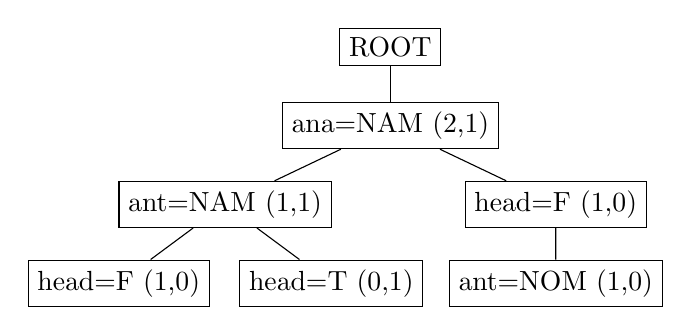
\begin{tikzpicture}
\node [rectangle,draw]{ROOT} [level distance=10mm,sibling distance=25mm]
child { node [rectangle,draw]{ana=NAM (2,1)} [level distance=10mm ,sibling distance=42mm]
child {node [rectangle,draw] {ant=NAM (1,1)}  [level distance=10mm ,sibling distance=27mm]
child {node [rectangle,draw] {head=F (1,0)}}
child {node [rectangle,draw] {head=T (0,1)}}
}
child {node [rectangle,draw] {head=F (1,0)}
child {node [rectangle,draw] {ant=NOM (1,0)}
}}
};
\end{tikzpicture}
\end{center}
\caption[The final FP-Tree with support values]{FP-Tree with corresponding support values of the nodes.\label{final-fp-tree_example}}
\end{figure*}
Figure~\ref{final-fp-tree_example} shows the resulted FP-Tree in which corresponding support values for 
both classes, i.e.\ zero and one, are also included in each node.
\begin{figure*}[!htb]
\begin{center}
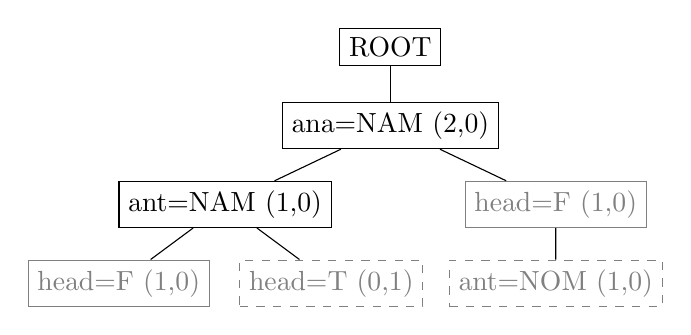
\begin{tikzpicture}
\node [rectangle,draw]{ROOT} [level distance=10mm,sibling distance=25mm]
child { node [rectangle,draw]{ana=NAM (2,0)} [level distance=10mm ,sibling distance=42mm]
child {node [rectangle,draw] {ant=NAM (1,0)}  [level distance=10mm ,sibling distance=27mm]
child {node [rectangle,draw,gray] {head=F (1,0)}}
child {node [rectangle,draw,gray,dashed] {head=T (0,1)}}
}
child {node [rectangle,draw,gray] {head=F (1,0)}
child {node [rectangle,draw,gray,dashed] {ant=NOM (1,0)}
}}
};
\end{tikzpicture}
\end{center}
\caption{Conditional FP-Tree for the $p=\{\text{head=F}\}$ pattern.\label{conditional-fp-tree_example_1}}
\end{figure*}
\begin{figure*}[!htb]
\begin{center}
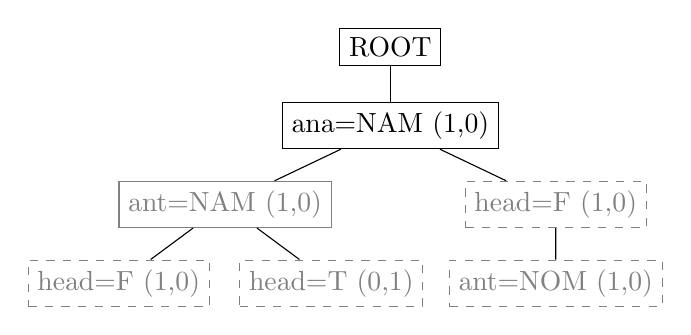
\begin{tikzpicture}
\node [rectangle,draw]{ROOT} [level distance=10mm,sibling distance=25mm]
child { node [rectangle,draw]{ana=NAM (1,0)} [level distance=10mm ,sibling distance=42mm]
child {node [rectangle,draw,gray] {ant=NAM (1,0)}  [level distance=10mm ,sibling distance=27mm]
child {node [rectangle,draw,gray,dashed] {head=F (1,0)}}
child {node [rectangle,draw,gray,dashed] {head=T (0,1)}}
}
child {node [rectangle,draw,gray,dashed] {head=F (1,0)}
child {node [rectangle,draw,gray,dashed] {ant=NOM (1,0)}
}}
};
\end{tikzpicture}
\end{center}
\caption{Conditional FP-Tree for the $p=\{\text{head=F},\text{ant=NAM}\}$ pattern.\label{conditional-fp-tree_example_2}}
\end{figure*}

Figure~\ref{conditional-fp-tree_example_1} and Figure~\ref{conditional-fp-tree_example_2} 
show the conditional FP-Trees that are built based on the FP-Tree of Figure~\ref{final-fp-tree_example} 
and for patterns $p=\{\text{head=F}\}$ and $p=\{\text{head=F},\text{ant=NAM}\}$, respectively.
%Gray nodes in conditional trees will be skipped from further processing.
%
\subsection{Discriminative Pattern Mining vs. Feature Selection}
In this paper, we used a discriminative pattern mining approach for determining feature-values 
that are informative for the coreference label when they are considered in combination.

An alternative approach would be to use a standard feature selection algorithm where each feature-value is considered as a feature.
There are three feature selection models: \emph{filter}, \emph{wrapper} and \emph{embedded}.

\emph{Wrapper} models use a learning algorithm, i.e.\ coreference resolver in our scenario, in the loop, and therefore assess the performance
of different feature subsets based on the performance of the learning algorithm on an evaluation set.
Wrappers are, however, 
computationally expensive in our scenario since they require the coreference resolver to be executed in
every iteration of the feature-value subset selection. For $n$ feature-values, there exist $2^n$ possible combinations. $n$ is around 500 in our data and deep-coref takes two days for training using GPUs.


\emph{Filter} models, on the other hand, are solely data dependent and therefore are independent of the learning algorithm.
The use of a discriminative pattern mining approach for informative feature-value selection, is equivalent to a filter model.

Finally, embedded models are
incorporated into the learning algorithm itself.
For instance, we can incorporate all possible feature-values in deep-coref and use 
various regularization methods, e.g.\ dropouts, l$_1$ and l$_2$ regularizations, instead of pre-selecting informative feature-values.
We examined the above regularization methods in ``top-pairs+linguistic'' experiments.
The use of each of the above regularizations on top of the feature layer in deep-coref
results in significantly lower performance than either of ``top-pairs'' and ``top-pairs+linguistic'' results on the CoNLL development set.
It is worth mentioning that we did not perform hyperparameter optimization for these experiments.
We examine $0.2$, $0.3$ and $0.5$ values for dropout and $0.01$ as the regularization parameter.
If we want to tune these parameters, the question would be the choice of the evaluation set since our main focus is to improve generalization. We leave this direction for future work.

Overall, it is worth noting that EPM uses an exhaustive search to explore all frequent combination of feature-values up to a certain length, unlike many existing feature selection algorithms that use heuristic algorithms for searching feature subsets.

\iffalse
\subsection{Basic Features}
Table~\ref{tab:feature-list} contains the list of basic features that are used in this paper.
\begin{table*}[!htb]
    \begin{center}\footnotesize
    \begin{tabular}{|l|l|l|}
    \hline
     \parbox[t]{2mm}{\multirow{9}{*}{\rotatebox[origin=c]{90}{Mention-based}}} 
     & mention type & proper name, nominal, pronominal and other \\
     & fine mention type & proper name, definite or indefinite nominal, or one of the 
 he, she, it, they, I, you, or we pronouns \\
 & gender & male, female, neutral, unknown\\
 & number& singular, plural, unknown\\ 
 & animacy & animate, inanimate, unknown\\
 & named entity type & extracted using Stanford NER \\
 & dependency relation & lexicalized dependency relation of the head word to its governor \\
 & POS tags & POS tags of the first, last, head, two preceding and two following words of each mention \\ \hline
 \parbox[t]{2mm}{\multirow{6}{*}{\rotatebox[origin=c]{90}{Pairwise}}} 
 & head match & the head words of two mentions match\\
 & acronym & one mention is the acronym of the other \\
 & string contained & the string of one mention is contained in the string of the other one \\
 & head contained & the head of one mention is contained in the string of the other one\\
 & compatible modifiers & mentions have not premodifiers or premodifiers of one mention are contained in those of the other \\ 
 & compatible gender & two mentions have the same gender or one of the gender values is unknown\\
 & compatible number& two mentions have the same number or one of the number values is unknown\\
 &compatible animacy& two mentions have the same animacy or one of the animacy values is unknown \\
     \hline
    \end{tabular}
    \end{center}
    \caption{The set of features that are used in our experiments.}
    \label{tab:feature-list}
\end{table*}
\fi
\iffalse
\subsection{Impact of Various Hyper-Parameters in EFM}
\begin{figure}[!htb]
\begin{center}
%\resizebox {\columnwidth} {!} {
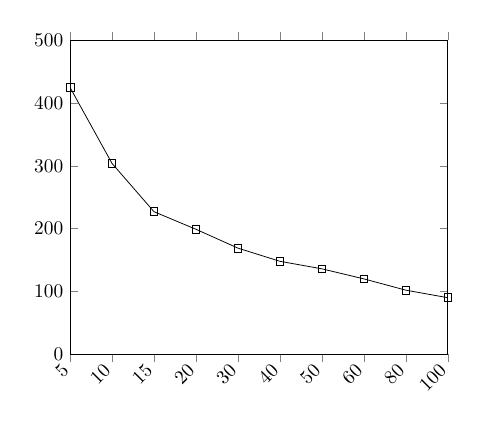
\begin{tikzpicture}[scale = .7]   %
\begin{axis}[
ymin = 0, ymax= 500, %ylabel = Mining Time (Seconds),
 draw=none,
 xtick=data,
 xticklabel = {\benchmark{\tick}},
 xtick align=outside,
 ytick align=inside,
 x tick label style={rotate=45,anchor=east},
 title style={font=\Large},
 ylabel near ticks,
 enlarge x limits=false,
xtick distance={400},
 symbolic x coords={5,10,15,20,30,40,50,60,80,100},
 ymajorgrids=true,
 grid = none,
 ]
\addplot[
    solid,
    color=black,
    mark=square,
    ]
    coordinates {
    (5,425)(10,304)(15,227)(20,199)(30,169)(40,148)(50,136)(60,120)(80,102)(100,90)
    };

 \end{axis}
\end{tikzpicture}
\end{center}
%}
\caption{The effect of the minimum support threshold on the number of resulting informative feature-values in EPM if $\Theta_l=5$.}
\label{fig:all}
\end{figure}

\begin{figure}[!htb]
\begin{center}
%\resizebox {\columnwidth} {!} {
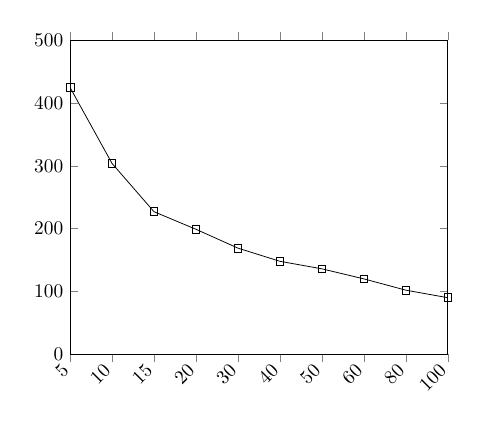
\begin{tikzpicture}[scale = .7]   %
\begin{axis}[
ymin = 0, ymax= 500, %ylabel = Mining Time (Seconds),
 draw=none,
 xtick=data,
 xticklabel = {\benchmark{\tick}},
 xtick align=outside,
 ytick align=inside,
 x tick label style={rotate=45,anchor=east},
 title style={font=\Large},
 ylabel near ticks,
 enlarge x limits=false,
xtick distance={400},
 symbolic x coords={5,10,15,20,30,40,50,60,80,100},
 ymajorgrids=true,
 grid = none,
 ]
\addplot[
    solid,
    color=black,
    mark=square,
    ]
    coordinates {
    (5,425)(10,304)(15,227)(20,199)(30,169)(40,148)(50,136)(60,120)(80,102)(100,90)
    };

 \end{axis}
\end{tikzpicture}
\end{center}
%}
\caption{The effect of $\Theta_l$ on the number of resulting informative feature-values in EPM if the minimum support is set to 20.}
\label{fig:all}
\end{figure}
\fi
 \begin{figure*}[!htb]
 \begin{minipage}{0.55\textwidth}
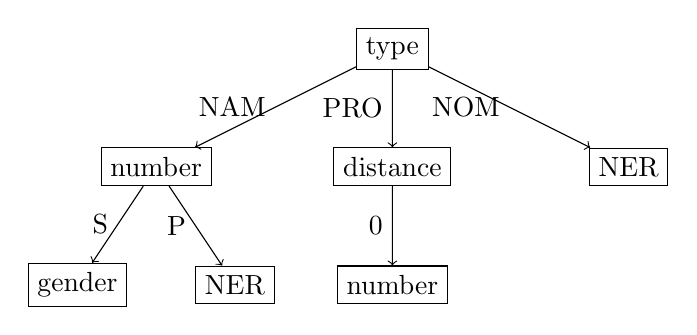
\begin{tikzpicture}
\node [rectangle,draw]{type} [level distance=15mm ,sibling distance=30mm]
child {node [rectangle,draw] {number}  [level distance=15mm ,sibling distance=20mm]
child {node [rectangle,draw] {gender}
edge from parent [->] node [left] {S}
}
child {node [rectangle,draw] {NER}
edge from parent [->] node [left] {P}
}
edge from parent [->] node [left] {NAM}
}
child {node [rectangle,draw] {distance}
child {node [rectangle,draw] {number}
edge from parent [->] node [left] {0}
}
edge from parent [->] node [left] {PRO}
}
child {node [rectangle,draw] {NER}
edge from parent [->] node [left] {NOM}
}
;
\end{tikzpicture}
 \end{minipage}
 \begin{minipage}{0.35\textwidth}
  \begin{itemize}
   \item[] type+number
   \item[] type+number+gender
   \item[] type+number+NER
   \item[] type+distance
   \item[] type+distance+number
   \item[] type+NER
  \end{itemize}

 \end{minipage}
\caption[A sample decision tree and its corresponding feature conjunctions]{A sample decision tree and the list of all extracted feature conjunctions based on Fernandes et al.'s (2012) approach. \label{fernandes_tree}}
\end{figure*}
\subsection{Example of Fernandes et al.'s (2012) Feature Templates}
Figure~\ref{fernandes_tree} shows a sample decision tree the list of corresponding feature templates that are extracted from it. 


\end{document}